\chapter{Carbon Dioxide Splitting}

\section{Traditional Process}

Before understanding the process of plasma-assisted CO$_2$ splitting, it would be useful to briefly explain the traditional thermally driven process. This process, sometimes referred to as pure CO$_2$ splitting, can take one of two possible forms. Often referred to as the reverse of coal burning, the overall reaction for CO$_2$ splitting can be written as:

\begin{equation}
    \ce{CO_2 -> C + O_2}
\end{equation}

This though is a simplification of the process, as it is most likely a two part mechanism \cite{rayne_2008}. The first half of the process would involve splitting the CO$_2$ into carbon monoxide (CO) and atomic oxygen (O) as seen in \ref{eq:co2_splitting}. The second step could take one of two possible pathways, however the most likely of the two would be the Boudouard reaction, seen in \ref{eq:boudouard_reaction}; however, this specific reaction is beyond the scope of this report.
%TODO: Need to add both reaction pathways

\begin{equation}
    \ce{2CO_2 -> 2CO + O_2}
    \label{eq:co2_splitting}
\end{equation}
\begin{equation}
    \ce{2CO -> C + CO_2}
    \label{eq:boudouard_reaction}
\end{equation}

Traditional thermal CO$_2$ splitting has not had much success to date, primarily due to the fact that CO$_2$ is an incredibly stable molecule with a Gibbs free energy of formation ($\Delta G^\circ$) of -394 kJ mol$^{-1}$. This is significantly higher than most other common gases as illustrated in figure \ref{fig:co2_stability}. 

\begin{figure}[h!]
	\centering
	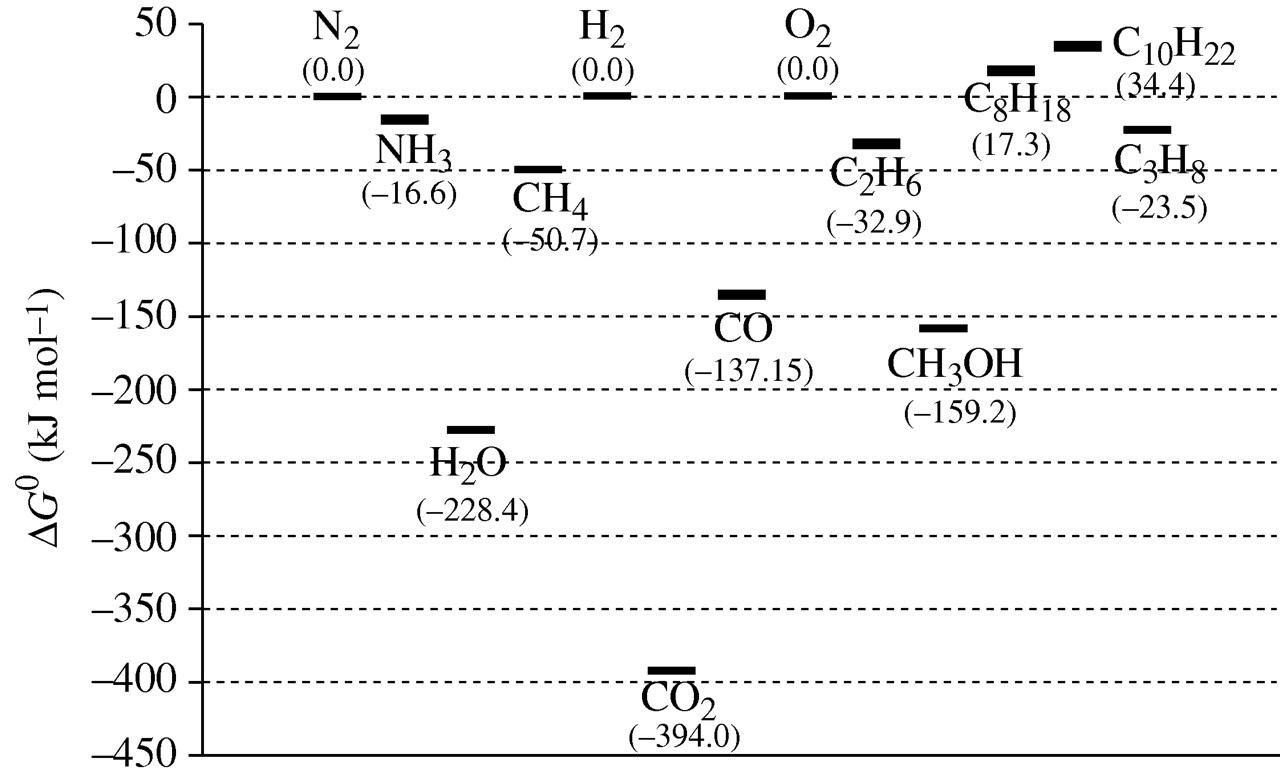
\includegraphics[width=0.6\linewidth]{chapter_3/figures/co2_stability.jpg}
	\caption{Gibbs free energy of formation for different chemicals based on data from the NIST database. \cite{jiang_xiao_kuznetsov_edwards_2010}}
	\label{fig:co2_stability}
\end{figure} 

The enthalpy of formation ($\Delta H^\circ_f$) of the reaction in \ref{eq:co2_splitting} is +283 kJ mol$^{-1}$, meaning that it is endothermic. Thus in order to make this reaction favourable, high temperatures are required. Figure \ref{fig:thermal_co2_conversion} highlights the conversion of such a reaction based on temperature, along with its corresponding energy efficiency \cite{Snoeckx2017}. This process could be improved by the presence of an active catalysts but this also increase the complexity and costs. 
%Alternatively, one could remove the reactants

\begin{figure}[h!]
	\centering
	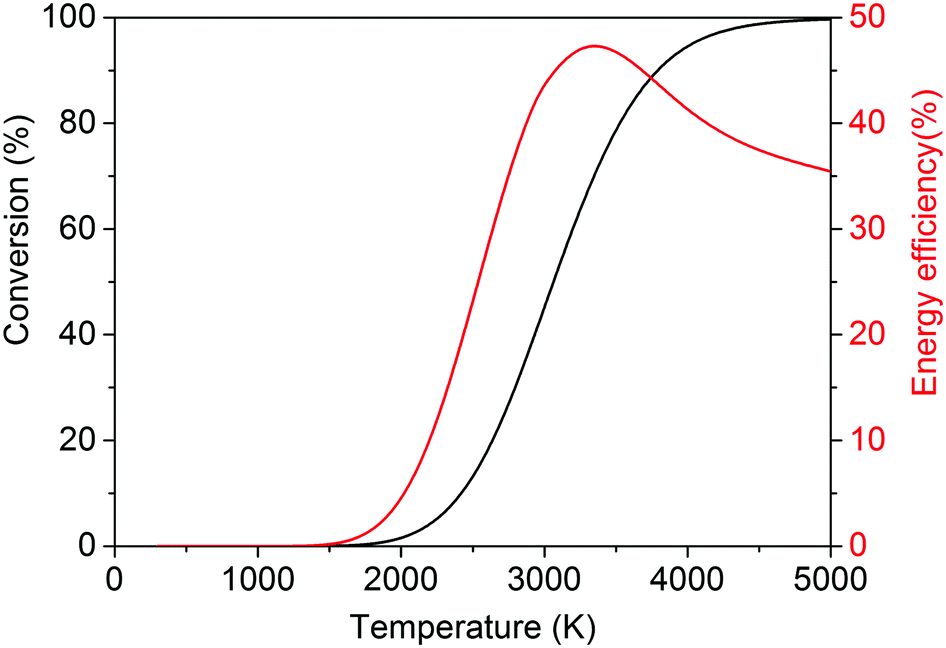
\includegraphics[width=0.6\linewidth]{chapter_3/figures/thermal_co2_conversion.png}
	\caption{Thermal conversion and energy efficiency of CO$_2$ splitting as a function of temperature. \cite{Snoeckx2017}}
	\label{fig:thermal_co2_conversion}
\end{figure}

Because of the low energy efficiency of pure CO$_2$ splitting, it is oftentimes more practical to include the use of a co-reactant. Ideally, this is done using a co-reactant with a higher Gibbs free energy (i.e. a less negative value) \cite{jiang_xiao_kuznetsov_edwards_2010}. In the literature, the most common co-reactants for CO$_2$ splitting are methane (CH$_4$, $\Delta G^\circ$ = -50.7 kJ mol$^{-1}$) and hydrogen (H$_2$, $\Delta G^\circ$ = 0.0 kJ mol$^{-1}$).

% TODO: Add reference for this
The CO$_2$ splitting with CH$_4$ is a reaction that generates synthesis gas (syngas), principally used in the production of ammonia and methanol \cite{}. The process is referred as the dry reforming of methane and can be expressed as: 

\begin{equation}
    \ce{CH_4 + CO_2 -> 2CO + 2H_2}
    \label{eq:drm}
\end{equation}

This reaction is also endothermic, with a $\Delta H^\circ_f$ = +247 kJ mol$^{-1}$, hence has to be run at high temperatures (between 1000 K to 1300 K, much lower than that of pure CO$_2$ splitting) and in the presence of a catalysts (typically nickel) \cite{pakhare_spivey_2014}. However, the big limitation with this process is the formation of soot on the catalyst, reducing the yields.

As for using H$_2$ as a co-reactant to CO$_2$ splitting, this process is known as the Sabatier reaction. The reaction, seen in \ref{eq:sabatier_reaction}, is typically to generate synthetic natural gas but has other uses such as the production of water on the international space station \cite{the_sabatier_system}.

\begin{equation}
    \ce{CO_2 + 4H_2 -> CH_4 + 2H_2O}
    \label{eq:sabatier_reaction}
\end{equation}

The reaction is exothermic, with a $\Delta H^\circ_f$ = -165.3 kJ mol$^{-1}$, but does require a catalyst in order to achieve high conversion yields. Nonetheless, there are two issues with this process. The first being, unless water is the desired end product, a third of the H$_2$ used goes towards the creation of a waste product; not ideal when using this process at scale. The other issues has to do with the fact that most of the world's supply of H$_2$ comes from the process of steam reforming, which produces CO$_2$ as a by-product. 

\section{Plasma-assisted $CO_2$ Splitting}

As highlighted above, there are several shortfalls with the traditional process of CO$_2$ splitting. This is where the use of plasma, specifically non-thermal plasmas (i.e. generated by electric means), can be beneficial. In these plasmas,  electrons have a higher temperature than the ions or the background gas. Energetic electrons in the plasma can dissociate molecules, even highly stable ones such as CO$_2$ at standard temperatures and pressures \cite{Snoeckx2017}. 

Because of this behaviour, there is no need for heat and pressurised reactors, reducing the complexity (and thereby costs). This leads on to the second benefit, where the entire operation of such a reaction is described as a 'turn-key' process due to the ability to instantly turn the plasma on and off, with minimal stabilisation times. There is also no need for rare earth metals to be used as catalysts, and it has been shown that plasma reactors can have good scalability as shown by Kogelschatz in \cite{kogelschatz_2003}.  

There are several different methods to generate plasma for CO$_2$ splitting in the literature, however the most common are: dielectric barrier discharges, gilding arc discharges, and radio frequency(RF)/microwave discharges. This report will only cover the RF/microwave discharges as it is the process being used, with several examples in the literature highlighted below.

\begin{figure}[h!]
	\centering
	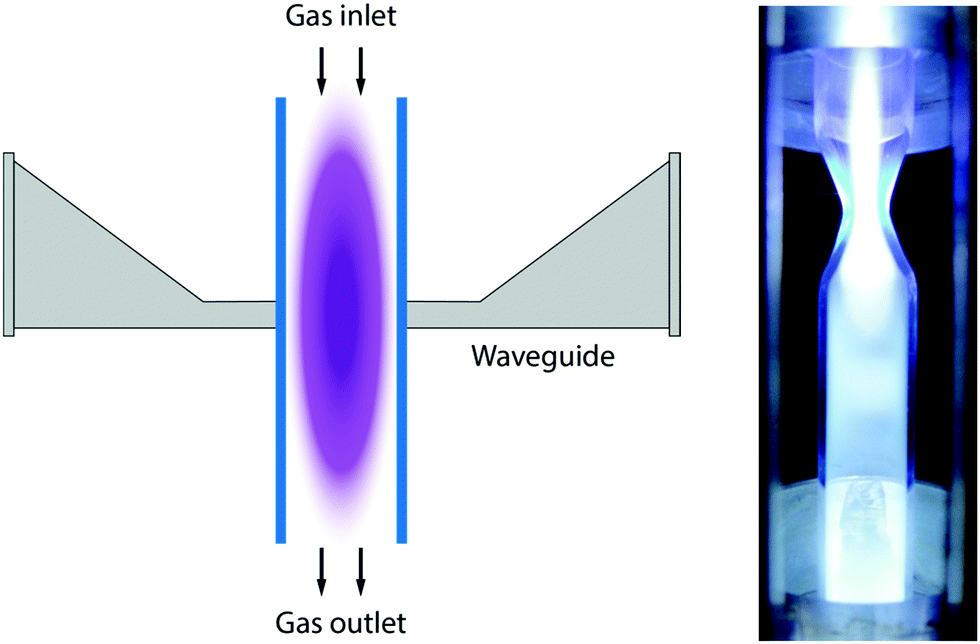
\includegraphics[width=0.6\linewidth]{chapter_3/figures/mw_reactor.png}
	\caption{Schematic of microwave reactors for CO$_2$ splitting. \cite{Snoeckx2017}}
	\label{fig:mw_reactor}
\end{figure}

Many experiments utilise a structure as seen in figure \ref{fig:mw_reactor}, whereby the gas is fed in via a quartz tube coupled with an external wave guide where the microwave discharge is generated. Such a design was used by Spencer and Gallimore \cite{spencer_gallimore_2010} to achieve a conversion efficiency of approximately 90\%; although this came at the cost of energy efficiency which reached a maximum of 3\%. The authors went on to state that such a system would not be suitable for  CO$_2$ emission reductions.

Nonetheless, other designs for RF/microwave discharges exist such as the one developed by Xu et al \cite{Xu2021}. Their design utilised a co-reactant called \textit{trans}-stilbene. Unlike the co-reactants previously mentioned, which were  gaseous, \textit{trans}-stilbene is a liquid. Because of this, the plasma had to directly contact the solution, which was achieved via a plasma jet reactor. The jet nozzle had to be place 4 mm above the surface of the liquid, and the final product of this reaction was CO and epoxides (a popular compound use for detergents, adhesives, and plastics). The authors were able to obtain a 75\% yield on epoxides and a splitting of approximately 70\% of the CO$_2$ in the plasma. As such, this will be the process that is emulated in this report.


